% !TEX root = ../main.tex
\subsection{FMT Alignment} \label{ssec::fmtalignment}
% WHY IS IT NEEDED
    While in a perfect world the target and each detector would be installed precisely where they are needed, in the real world there is an unavoidable misalignment in their positions.
    This misalignment needs to be addressed and included into reconstruction:
    the software needs to be aware of where a detector is positioned in relation to the target to provide meaningful results.
    
    In the CLAS collaboration, the Calibration and Commissioning group (CalCom) is in charge of the alignment and calibration of each detector.
    Shifts and rotations that need to be applied for alignment are included in the Calibration and Conditions Database (CCDB), which is then read in reconstruction. % NOTE. A CITATION HERE WOULD BE COOL.
    
    The main goals of alignment work were three:
    First, to provide FMT alignment tables to Run Group F (RG-F) so that they may be used in reconstruction.
    Second, to check if the resolution improvement from FMT is good enough to justify the extra material added to the CLAS12 detector.
    Finally, to provide detailed information about these improvements so that Run Group E (RG-E) and other run groups can choose if they will include the detector to their runs.

% DEFINITIONS
    Alignment shifts can be made in any of the three global axes:
    $z$, which is concentric to the beamline, $x$, which is parallel to the ground, and $y$, which points up from the ground.
    Then, alignment rotations can be done in any of these axes, and for the purposes of this work will be referred to as $\phi$ rotation (roll), when they're done around the $z$ axis, and pitch and yaw when they're done around the $x$ and $y$ axes respectively.
    
    To measure misalignment, we define a the Distance Of Closest Approach (DOCA) between a reconstructed DC track and an FMT cluster as a \textbf{Residual}.
    Due to each layer's geometry (refer to figure \ref{fig::fmt_geometry}), only the residuals in a layer's local $y$ axis (perpendicular to the strips) can be measured.
    This means that global $z$ and $\phi$ alignment can be done for each layer independently, but global $x$, global $y$, pitch, and yaw alignment has to be done for the entire detector at once.

% HOW WAS IT DONE
    \begin{figure}[b!]
        \centering\frame{
        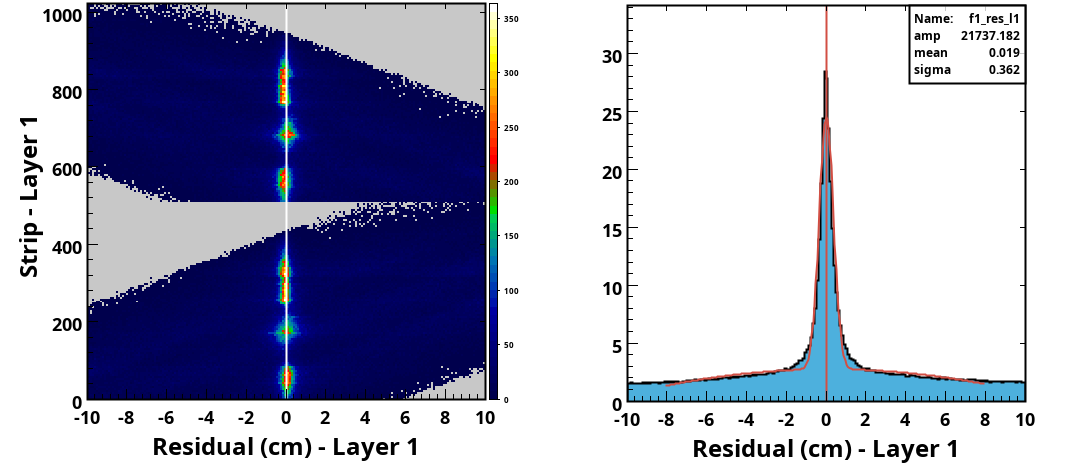
\includegraphics[width=\textwidth]{12fmtalign/img/20res_example.png}}
        \caption{Example residuals plot.}
        \label{fig::res_example}
    \end{figure}

    To minimise residuals, they are plotted for a particular shift or rotation in any of the relevant axes.
    An example of such a plot is shown in figure \ref{fig::res_example}.
    Since a Gaussian distribution is to be expected for the residuals, a Gaussian fit is applied to them.
    For $z$ and $\phi$ alignment, the goodness of a fit is evaluated heuristically by comparing their $\sigma$ and choosing the shift with the minimum $\sigma$.
    Then, for $x$, $y$, pitch, and yaw alignment, the goodness of a fit is evaluated heuristically by choosing the fit with the mean closest to $0$.
    The minimums are of course chosen within a healthy error margin.
    Examples of $z$ and $xy$ goodness of fit distributions can be seen in figure \ref{fig::resfit_example}.
    
    \begin{figure}[t!]
        \centering\frame{
        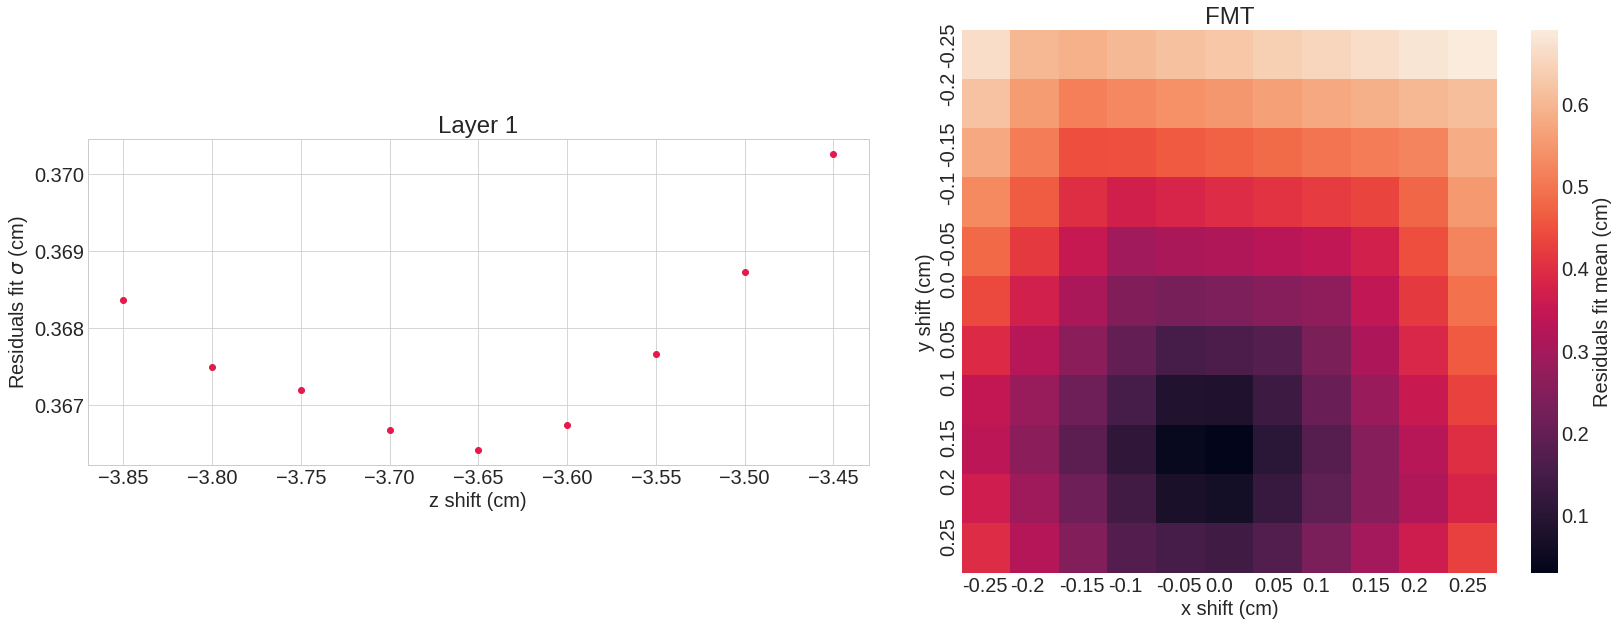
\includegraphics[width=\textwidth]{12fmtalign/img/20resfit_example.png}}
        \caption{Examples of residuals goodness of fit plots.}
        \label{fig::resfit_example}
    \end{figure}

\subsubsection{Fiducial Cuts}
    To reduce background, fiducial cuts are applied to the DC tracks and FMT clusters.
    This process is useful to increase data quality in order to obtain meaningful alignment results.
    
    For DC tracks, the cuts applied are:
    \begin{itemize}
        \item $\text{track}.z < \text{layer}.z$:
        Remove tracks with a vertex $z$ further downstream than the FMT layer before swimming.
        This is caused by reconstruction errors where the particle origin is outside of the target.
        % $9.84\%$ of tracks fail to meet this criterion in the sample data.
        \item $\mid\text{track}.z - \text{layer}.z\mid < 0.05 \text{cm}$:
        Remove tracks too far from the FMT layer after swimming.
        This was caused by bugs in the swimmer which will be mentioned in the next section.
        % $18.67\%$ tracks failed to meet this criterion.
        \item $5 \text{cm} < \sqrt{x^2 + y^2} < 25 \text{cm}$:
        Remove tracks outside of the layer's active region.
        % $35.22\%$ of the tracks were lost to this criterion.
        \item $\theta < ~66.42^{\circ}$:
        Remove tracks with a $\theta$ angle too high.
        When this happens, the same particle is affecting many strips, which causes the detector's data to not be as reliable as we want for alignment.
        % $7.22\%$ of tracks were lost to this criterion.
    \end{itemize}
    % From all these criteria, $70.95\%$ of the DC tracks were lost.
    % It is worth noting that after some reconstruction errors were fixed (as will be detailed in the following section), this percentage was reduced to $52.28\%$.
    
    For FMT clusters, the cuts applied are:
    \begin{itemize}
        \item $50 \text{ns} < \text{T}_{\text{min}} < 500 \text{ns}$:
        Cut clusters with an illogical $\text{T}_{\text{min}}$, which is the time of the first hit in the cluster.
        % $21.12\%$ of clusters fail to meet this criterion.
        \item $\text{size} > 1$ $\&\&$ $\text{E} > 100$:
        Cut small clusters with high energy, which are generally considered bad.
        % Only $7.36\%$ clusters are lost to this criterion.
        \item $\text{size} < 5$:
        Cut large clusters, which are not considered very useful.
        % Only $7.77\%$ are lost to this criterion.
    \end{itemize}
    % From all these criteria, $36.25\%$ of the FMT clusters were lost.

% RESIDUALS IMPROVEMENT
\subsubsection{Residuals Improvements}
    To validate the alignment algorithm proposed, it was tested on RG-F data (run $\mathbf{11983}$).
    The improvement in residuals is immediately obvious, as can be seen in figure \ref{fig::res_comparison}, noting the difference in scale between the top and bottom plots.
    
    \begin{figure}[t!]
        \centering\frame{
        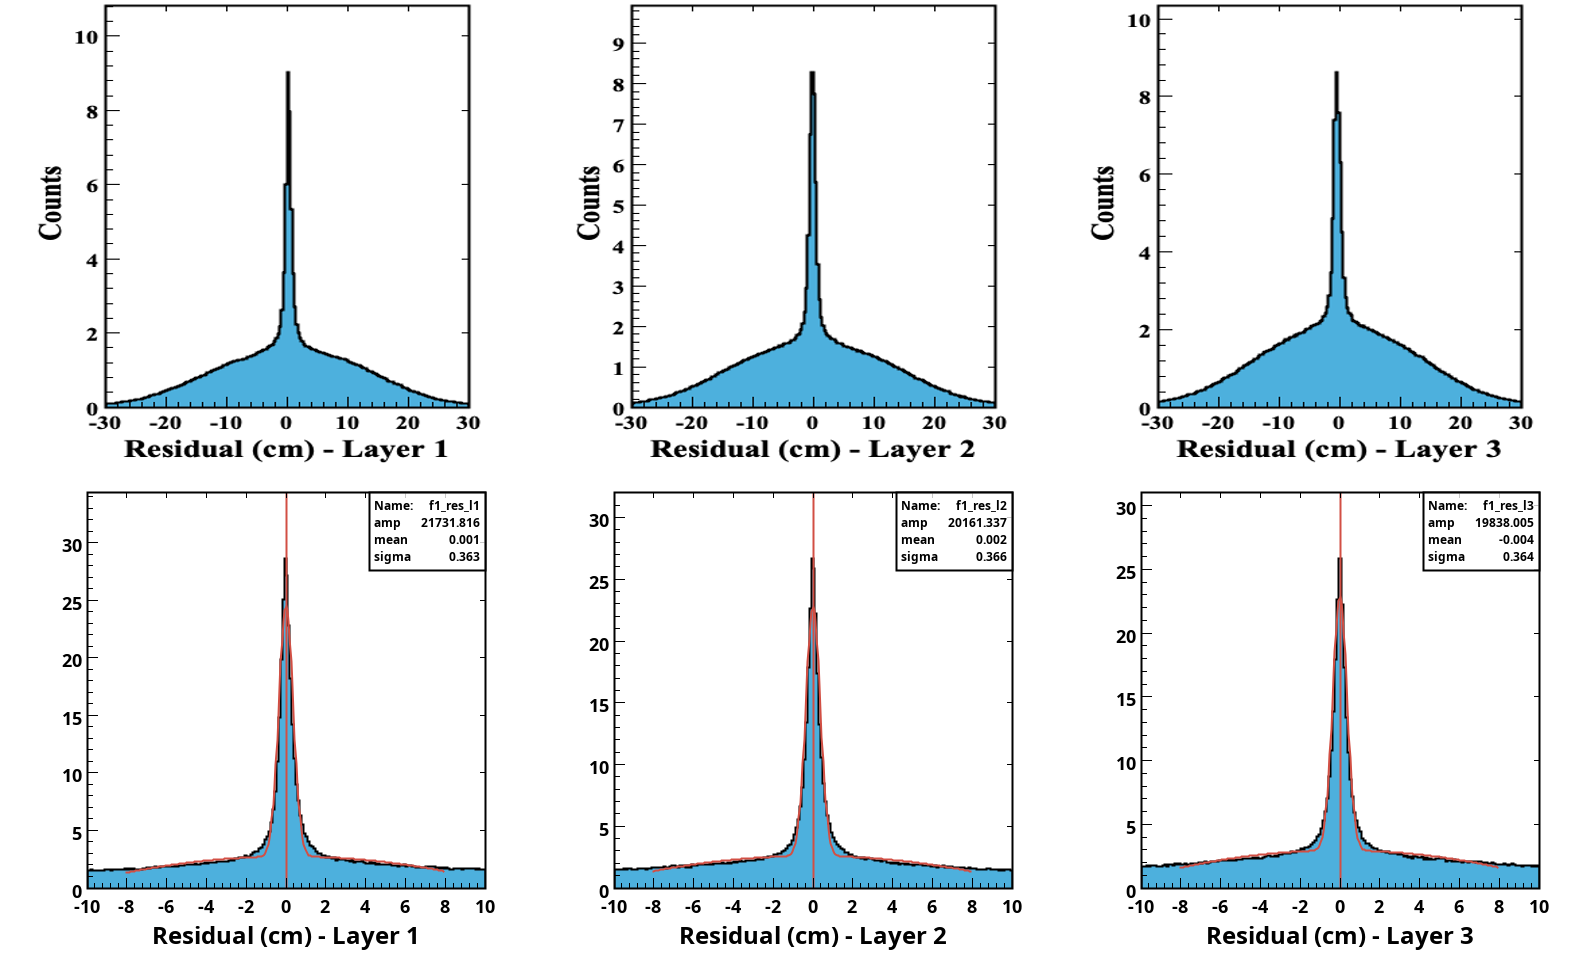
\includegraphics[width=\textwidth]{12fmtalign/img/20res_comparison.png}}
        \caption[Residuals distribution improvement.]{Residuals distribution before (upper image) and after (lower image) alignment.}
        \label{fig::res_comparison}
    \end{figure}
    
    As can be seen in the figure, the $z$ and $\phi$ alignment heavily reduces the background, increasing the number of residuals near the mean of the distribution.
    In addition, the $x$ and $y$ alignment pushes this mean to zero, whereas it was slightly off before.
    Finally, no meaningful results were obtained for pitch and yaw alignment.
    This is attributed to how small the rotations around the $x$ and $y$ axes are, compounded with the fact that three layers do not provide enough data to perform alignment precise enough.
    
    To measure the mean and $\sigma$ of the distribution, a Gaussian fit was used.
    Its parameters are
    
     \begin{align*}
        \Big( \text{amp} \cdot \text{gaus}(\mu, \sigma) \Big) &+ \Big( p_0 + p_1\cdot x + p_2\cdot x^2 \Big) \\
        \text{gaussian} \hspace{0.8cm} &+ \hspace{1cm} \text{background}
    \end{align*}

    The results obtained are included in the CCDB at:
    
    \small\href{https://clasweb.jlab.org/cgi-bin/ccdb/versions?table=/geometry/fmt/alignment}{\texttt{clasweb.jlab.org/cgi-bin/ccdb/versions?table=/geometry/fmt/alignment}}
    
    Alignment was also later performed for Run Group M (RG-M) data successfully, proving that the alignment procedure is agnostic to a particular run.
    How this alignment procedure affects the resolution of the entire CLAS12 detector will be explored at the end of the chapter.

    The procedure described in this section is documented and shared publicly.
    It can be seen at:
    
    \href{https://github.com/JeffersonLab/clas12alignment/tree/master/fmt}{\texttt{github.com/JeffersonLab/clas12alignment/tree/master/fmt}}
